\section{Результаты}
В данной главе представлены результаты применения разработанного метода сегментации ледового канала с использованием нейросети. 
На маске, являющейся выходом нейросети, присутствуют три класса: вода, ледяное сало и лёд. Вода в объединении с ледяным салом 
формируют канал. Несмотря на определенные достижения, итоговый подход оказался неидеальным. Далее приведены основные метрики качества полученных результатов.

\subsection{Метрики}

Для оценки эффективности работы нейросети были использованы метрики полнота (recall) и точность (precision) для каждого класса отдельно, а также для канала в целом. 
\[Recall = \frac{TP}{TP + FN}; Precision = \frac{TP}{TP + FP}\]
Здесь $TP$ --- истинно положительный результат, $FN$ --- ложно отрицательный, $FP$ --- ложно положительный. Полнота позволяет понять долю правильно классифицированных 
пикселей из всех пикселей данного класса, в то время как точность отвечает за долю правильно классифицированных пикселей из всех пикселей, 
классифицированных в данный класс.
Результаты оценки приведены в Таблице~\ref{tab:nn_results}.
\begin{table}[h]
    \centering 
        \begin{tabular}{|c|c|c|} 
            \hline
            & Полнота & Точность \\
            \hline
            Вода & 0.64 & 0.47 \\ \hline
            Ледяное сало & 0.48 & 0.51 \\ \hline
            Канал & 0.86 & 0.61 \\ \hline
        \end{tabular}
    \caption{Качество маски}\label{tab:nn_results}
\end{table}

Из таблицы видно, что Recall для воды составил 0.64, а Precision — 0.47, что указывает на относительно высокую способность модели обнаруживать воду, 
но при этом значительное количество ложно положительных срабатываний. Аналогично, для ледяного сала метрики составили 0.48 и 0.51 соответственно, что также 
указывает на неполное соответствие предсказаний и истинных значений.

Однако не смотря на низкие метрики у каждого класса по отдельности, канал в целом выделяется удачно, хотя и с большим количеством ложных классификаций. Это достигается 
тем, что нейросеть иногда классифицирует воду, как ледяное сало и наоборот, что негативно сказывается на метриках этих классов, но никак не влияет на метрику канала в целом.

\subsection{Пример маски}

Для демонстрации полученных результатов на Рис.~\ref{fig:nn_mask} представлен пример маски канала, полученной в ходе сегментации.

\begin{figure}[htbp]
    \centering
    \subfloat[Изначальное изображение]{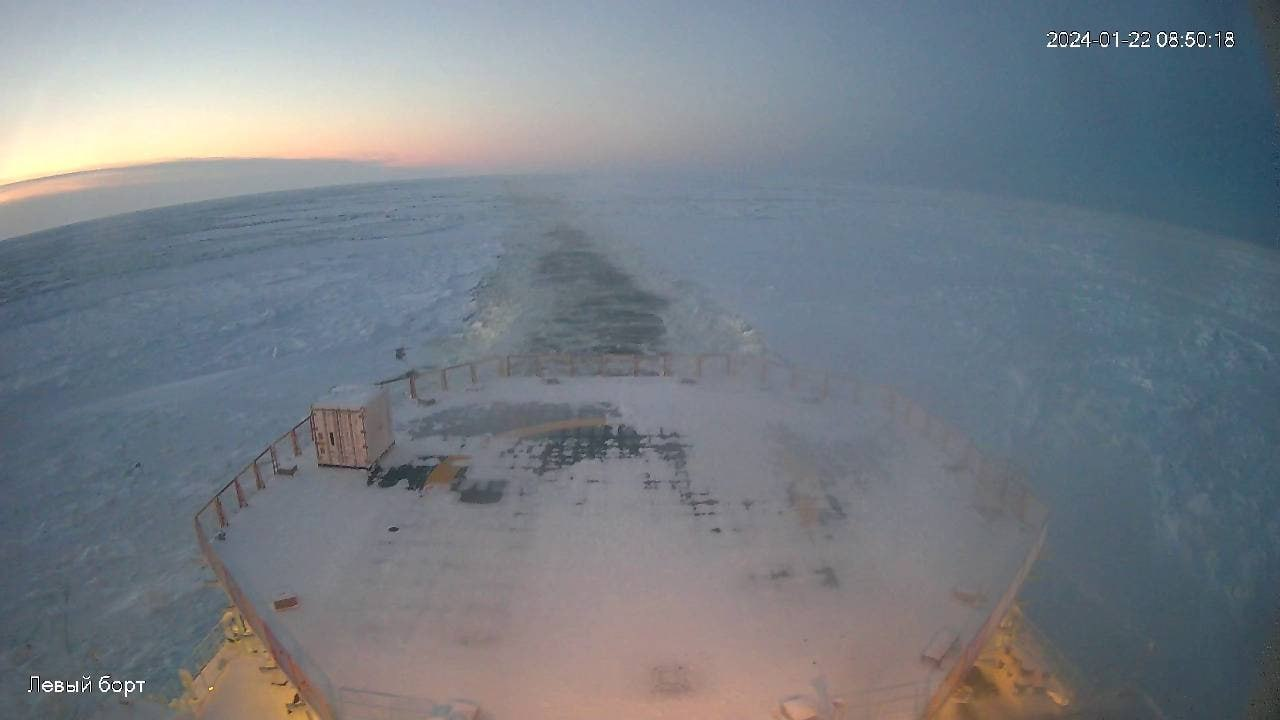
\includegraphics[scale=0.2]{src/Testing/assets/raw.jpg}}
    \subfloat[Маска нейросети]{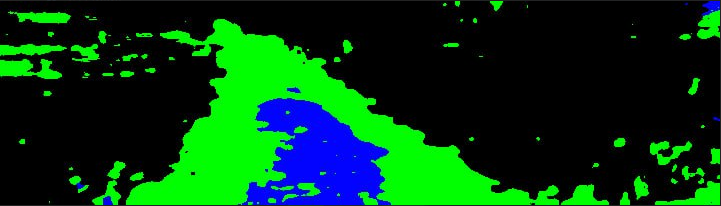
\includegraphics[scale=0.2]{src/Testing/assets/mask.png}}
    \\
    \caption{Результат работы нейросети}\label{fig:nn_mask}
\end{figure}

Здесь отображены области, отнесенные к трём классам: вода (синий цвет), ледяное сало (зелёный цвет) и лёд (чёрный цвет). 
Объединение синих и зеленых областей формирует сегментированный канал. Как видно из примера, нейросеть успешно выявляет основные контуры канала, 
однако присутствуют некоторые неточности и ложноположительные области.

\subsection{Итог}

Результаты сегментации показали, что разработанный метод способен достаточно эффективно выявлять ледовый канал позади ледокола. 
Высокий Recall канала (0.86) свидетельствует о том, что метод корректно идентифицирует большинство участков канала. 
Однако, относительно низкий Precision (0.61) указывает на наличие ложных положительных определений.

В целом, предложенный метод сегментации продемонстрировал свою применимость для выделения ледового канала, но он требует дополнительной фильтрации результатов, 
которая описана в главе выше.
